% This is LLNCS.DEM the demonstration file of
% the LaTeX macro package from Springer-Verlag
% for Lecture Notes in Computer Science,
% version 2.4 for LaTeX2e as of 16. April 2010
%
\documentclass{llncs}
%
\usepackage{makeidx}  % allows for indexgeneration
%
\usepackage{todonotes}
%
\usepackage{booktabs}
\usepackage{graphicx}

% http://mirror.utexas.edu/ctan/obsolete/macros/latex/contrib/subfigure/subfigure.pdf
\usepackage[tight]{subfigure}

\begin{document}
%
\frontmatter          % for the preliminaries
%
\pagestyle{headings}  % switches on printing of running heads
\addtocmark{Alpha Shapes for Tumor Inclusion} % additional mark in the TOC
%

%
\tableofcontents
%
\listoftodos

\mainmatter              % start of the contributions
%
\todo[author=SG,inline]{Change title and running title}
\title{Lung Segmentation via Alpha Shapes in the presence of large tumors}
%
\titlerunning{Alpha Shape Lung Segmentation}  % abbreviated title (for running head)
%                                     also used for the TOC unless
%                                     \toctitle is used
%
\todo[author=All, inline]{\\citep command available for parenthesis citation with natbib}
\todo[author=SG, inline]{Make anonymous}
\author{Sarah E. Gerard\inst{1} \and Hans J. Johnson\inst{1}
\and John Bayouth \and Kaifang Du \and Junfeng Guo \and Joseph M. Reinhardt\inst{1}}
%
\authorrunning{Sarah E. Gerard et al.} % abbreviated author list (for running head)
%
%%%% list of authors for the TOC (use if author list has to be modified)
\tocauthor{Sarah E. Gerard, Hans J. Johnson, Joseph M. Reinahrdt}
%
\institute{University of Iowa, Iowa City IA 52402, USA,\\
\email{sarah-gerard@uiowa.edu}}
\institute{Iowa Institute for Biomedical Imaging, Iowa City IA 52402, USA}


\maketitle              % typeset the title of the contribution

\begin{abstract}
Lung segmentation is a critical initial step for radiation therapy interventions of lung cancer patients. However, automatic segmentation of lungs with large tumors is a challenging task due to the large variation of both lung and tumor shape between subjects. We present a method to segment lungs with large tumors in CT images using an initial intensity based segmentation followed by alpha shape construction and graph search. We evaluated our method on twelve subjects. Compared to manual segmentations, we obtained an average DICE coefficient of 0.970 and an average surface distance of 0.809 mm. The results show that our method is able to accurately include large tumors. Additionally, when the method is performed on lungs with no tumors the initial lung segmentation is not significantly changed. 

\keywords{segmentation, alpha shapes, lung}
\end{abstract}
%
\section{Introduction}
%
Radiation therapy interventions of lung cancer patients involve acquiring a thoracic CT scan. Typically a respiratory correlated scan, or 4D CT, is also acquired prior to treatment. This produces a huge amount of data, requiring automatic computer-aided methods for further analysis. Accurate delineation of the lungs is a critical initial first step for treatment planning and quantitative analysis.

Normal lungs have high contrast with the surrounding anatomy, making lung segmentation relatively trivial using thresholding based methods ~\cite{guo2008,hu2001}. However, in the presence of large tumors, conventional threshold based methods fail because tumors are excluded from the segmentation. 

Several approaches have been used to segment pathological lungs. Statistical shape models are able to capture the major modes of lung shape variation in a training set and then build a lung model ~\cite{sun2012,sofka2011}. This method requires a large training set with annotated corresponding landmark points. Additionally, the training set is limited to a subset of possible lung shape variations and thus it could fail on cases that are not represented in the training set. Segmentation by registration methods ~\cite{sluimer2005,vanrikxoort2009} make use an atlas or multiple atlases with ground truth segmentations. The atlas segmentation is mapped to a test case using image registration. For good results, a time consuming registration is needed.

In this paper we propose an alpha shape approach for inclusion of large tumors in lung segmentations. Alpha shapes have been used for \todo[author=SG,inline]{need description of how alpha shapes used XXXXX}. To the best of our knowledge this is the first time alpha shapes have been used for inclusion of large tumors for lung segmentation. 


%
\section{Methods}
%
The proposed method has three main steps: initial intensity based segmentation, alpha shape computation of initial mask, and an optimal graph search for final refinement. Each of these steps will be described next.
%
\subsection{Initial Segmentation}
%

First we obtain intensity based segmentation of the lungs using PASS software ~\cite{guo2008}. This method consists of three main steps: extraction of lungs using optimal thresholding, separation of the right and left lungs, and optimal smoothing to smooth the lung boundaries. This gives a lung mask for both left and right lung, however large tumors are not included. We will refer to this as the initial mask. The next steps will process initial mask for the left and right lung separately. 
%
\subsection{Alpha Shapes}
%
\todo[author=SG,inline]{Make this section better}
The concept of using alpha shapes to represent a point set was originally presented in ~\cite{edelsbrunner1983}.
Given a finite set of points $P \epsilon \mathbb{R}^3$ and $ 0 \leq \alpha \leq \infty $ an $\alpha$-shape can be used to represent the shape of $P$. If $\alpha=\infy$ the $\alpha$-shape is equivalent to the convex hull. For decreasing $\alpha$, the $\alpha$ shape size gradually decreases until only $P$ remains at $\alpha=0$. The result is a family of shapes that can be used to represent $P$.

The boundary of the $\alpha$-shape is a subset of the Delaunay triangulation of points $P$. The Delaunay triangulation $T$ of $P$ is the a triangulation where the circumsphere of each d-simplex $t \epsilon T$ is empty, i.e. there are no  $p \epsilon P$ inside the circumsphere. This is the dual graph of the Voronoi diagram. The $\alpha$-shape is equivalent to the union of all $t \epsilon T$ s.t. the circumsphere of d-simplex $t \leq \alpha$. 

The lung shape is approximately convex along the pleural surface, so the convex hull of the initial mask gives a good estimate of the boundary for this surface.
 However, regions near mediastinum and diaphragm are not convex resulting in over over. Using alpha shapes we were able to elegantly obtain a family of shapes representing the initial mask. 


Our goal is to find the alpha shape of the initial lung mask that includes the tumor region. First we obtain a set of points representing the initial mask. The convex hull, or alpha shape with $ \alpha = \infty $, of the initial mask includes the tumor region however it also over segments non convex regions on the lung such as the mediastinum and diaphragm. By reducing alpha we can exclude most of the over segmentation near mediastinum and diaphragm. If alpha is too small, the tumor region is excluded. Figure ~\ref{fig:alphashapes} shows the alpha shape of the initial mask for different values of alpha. 

%
% http://texblog.org/2007/08/28/placing-figurestables-side-by-side-subfigure/
%
\begin{figure}[ht!]
  \centering
  \subfigure[CT]{
  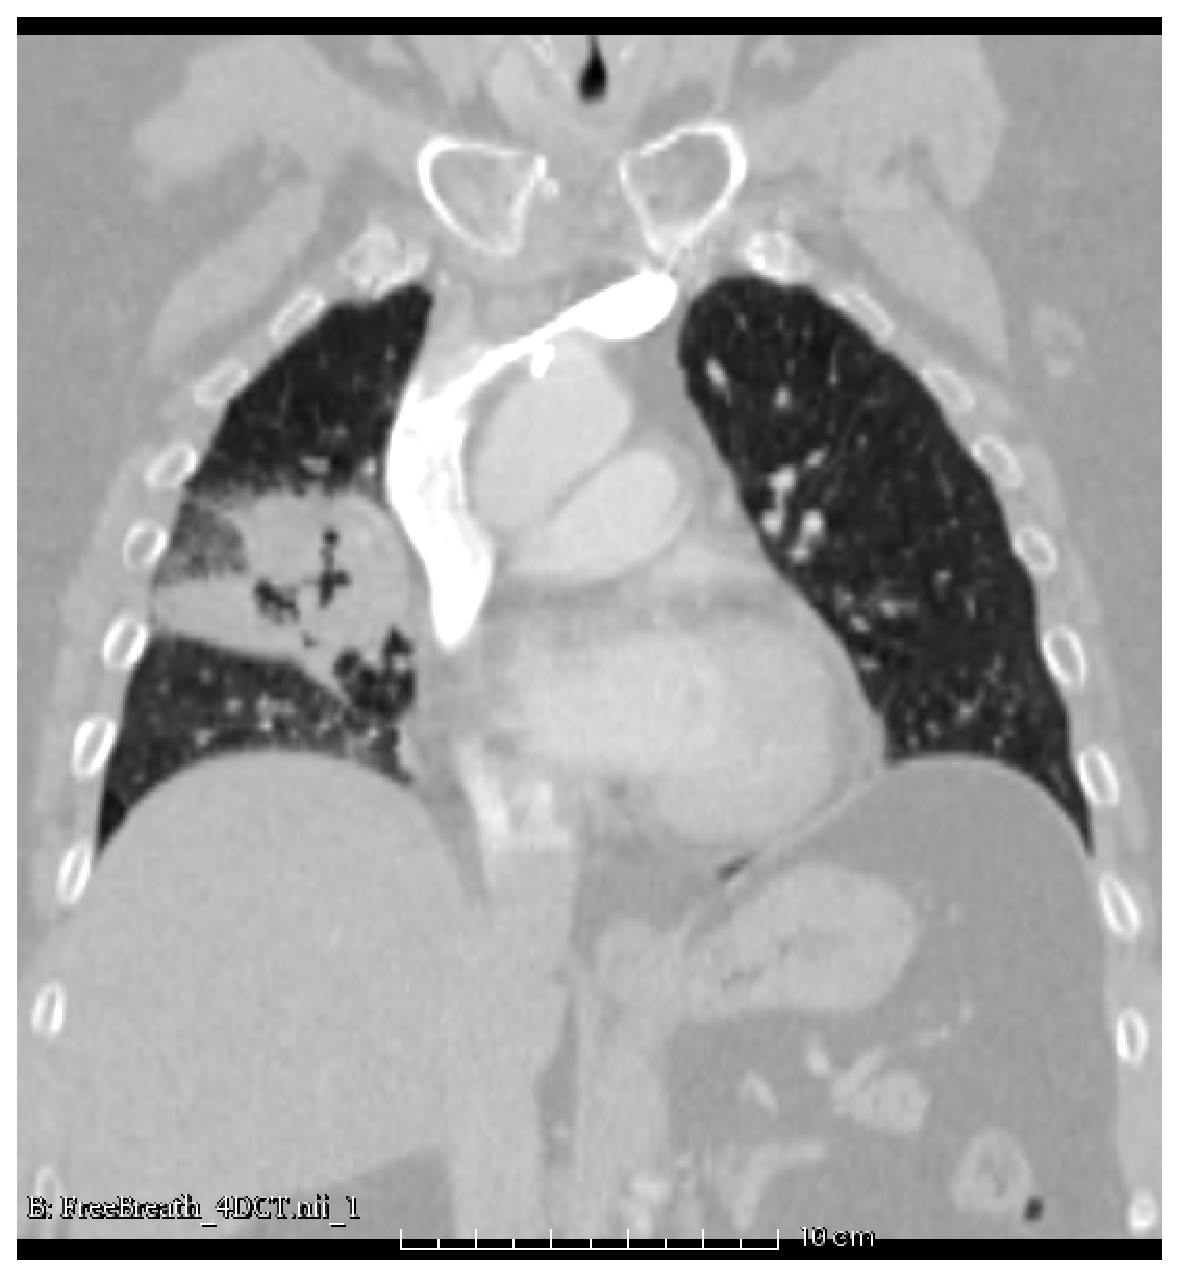
\includegraphics[trim={5 160 340 110},clip,width=1.0in, height=1.4in]{figs/ct}
  \label{fig:tris_CT}
  }
  \subfigure[Mask]{
  
\includegraphics[trim={5 150 300 100},clip,width=1.0in, height=1.4in]{figs/pass}
  \label{fig:tris_Mask}
  }
  \subfigure[Point Set]{
  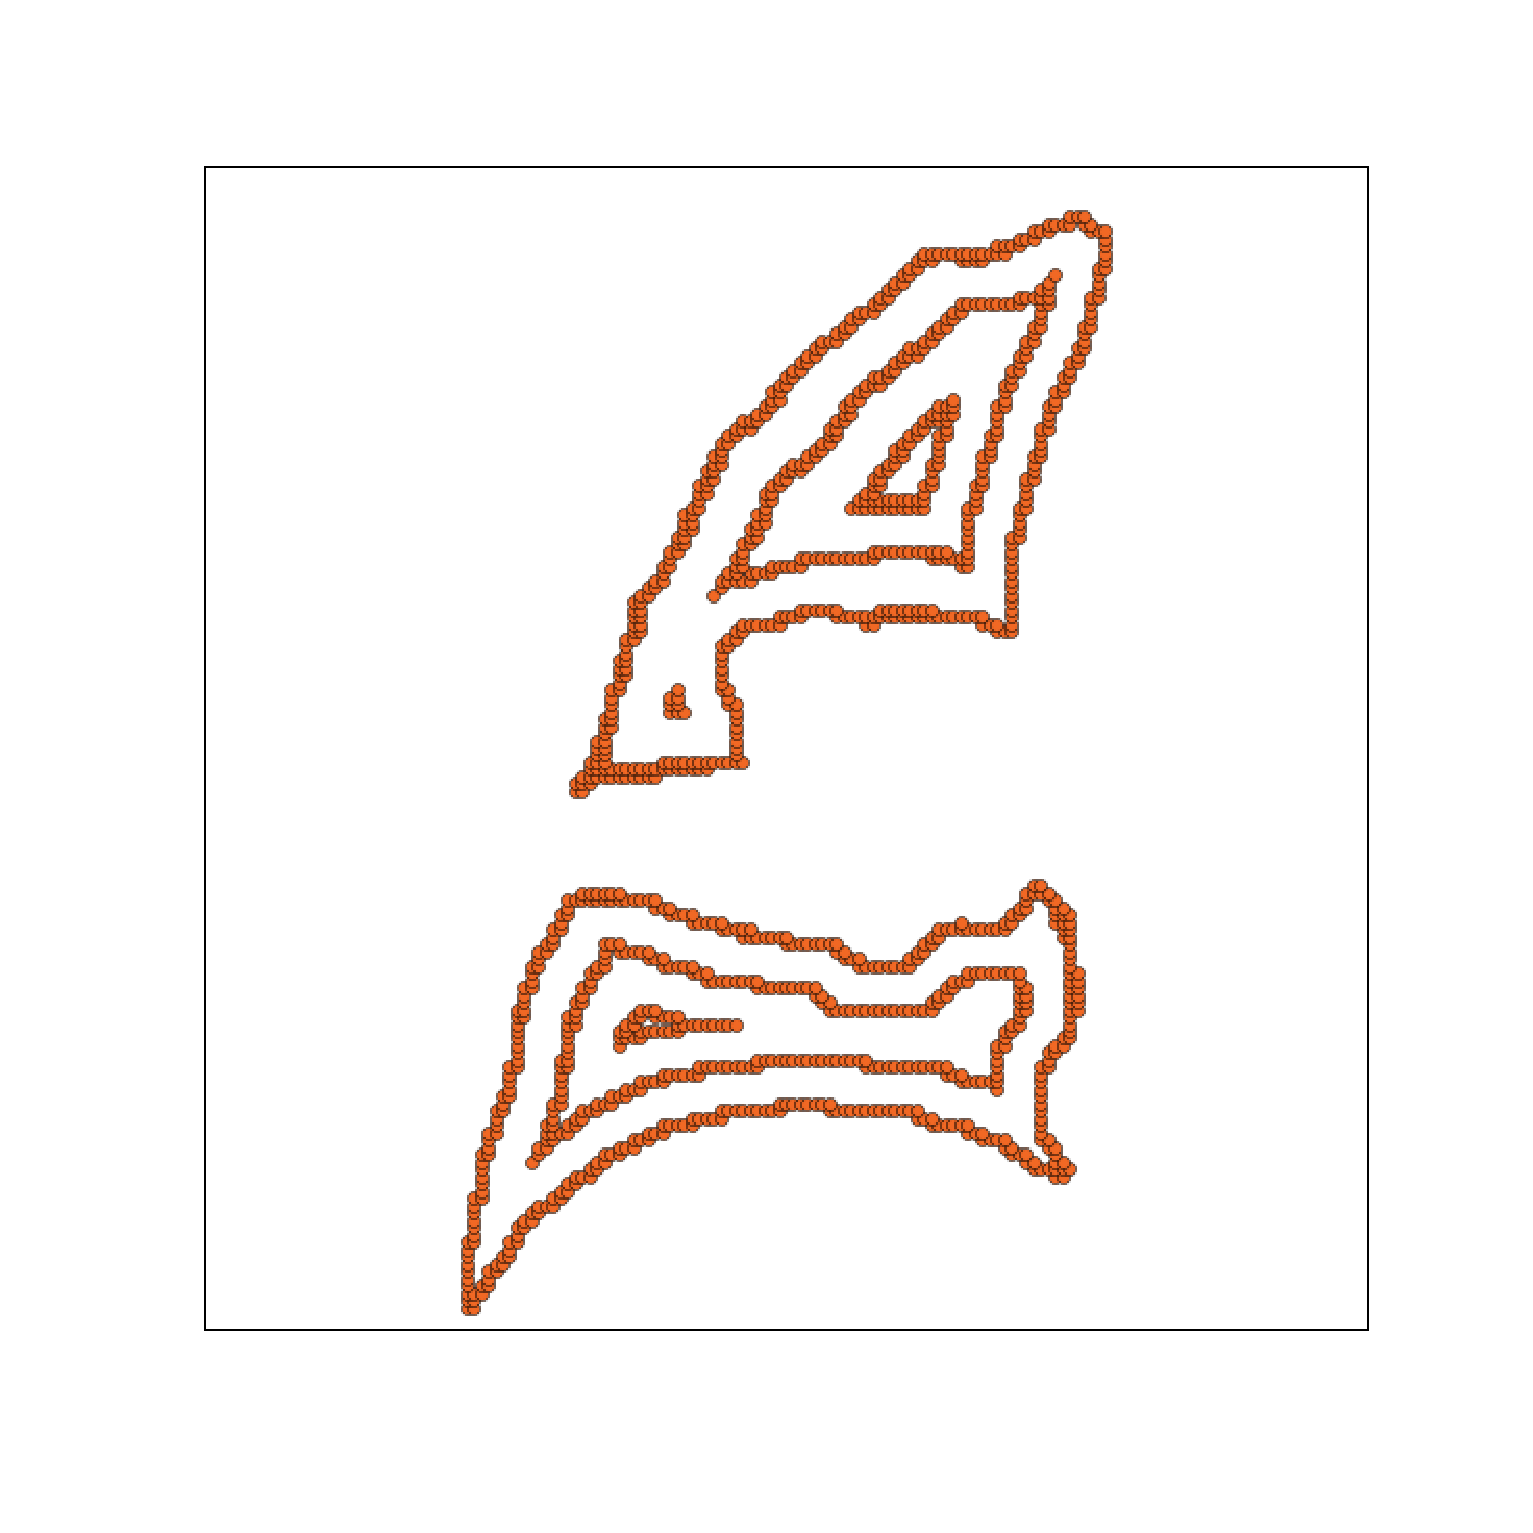
\includegraphics[trim={150 100 150 100},clip,width=1.0in]{figs/points}
  \label{fig:tris_points}
  }
  \subfigure[$\alpha = 200$]{
  \includegraphics[trim={150 100 150 100},clip,width=1.0in]{figs/tris_200}
  \label{fig:tris_alpha_200}
  }
  \subfigure[$\alpha = 66$]{
  \includegraphics[trim={150 100 150 100},clip,width=1.0in]{figs/tris_66}
  \label{fig:tris_alpha_66}
  }
  \subfigure[$\alpha = 50$]{
  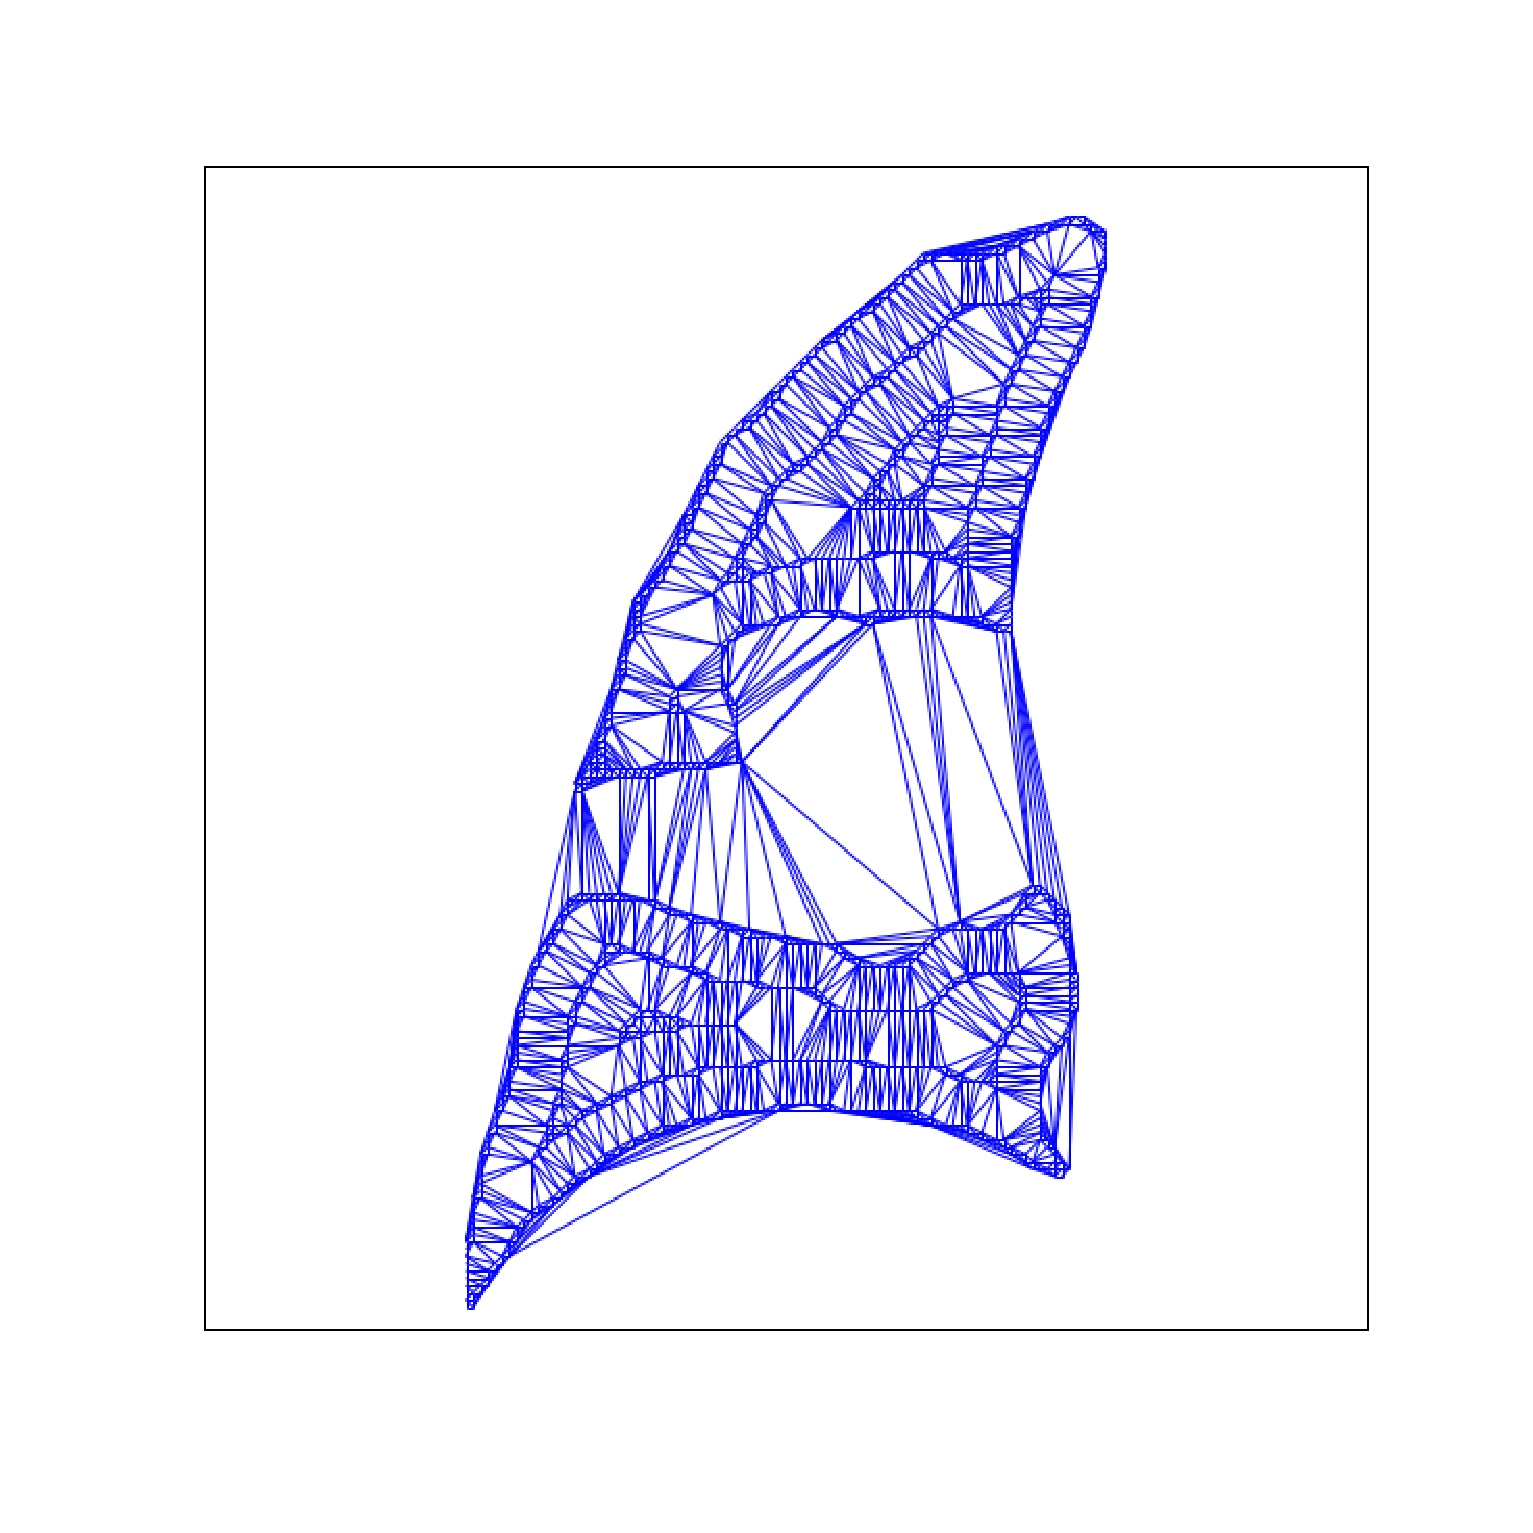
\includegraphics[trim={150 100 150 100},clip,width=1.0in]{figs/tris_50}
  \label{fig:tris_alpha_50}
  }
  \subfigure[$\alpha = 33$]{
  \includegraphics[trim={150 100 150 100},clip,width=1.0in]{figs/tris_33}
  \label{fig:tris_alpha_33}
  }
  \subfigure[$\alpha = 15$]{
  \includegraphics[trim={150 100 150 100},clip,width=1.0in]{figs/tris_15}
  \label{fig:tris_alpha_15}
  }

%  \begin{tabular}{cccc}
%    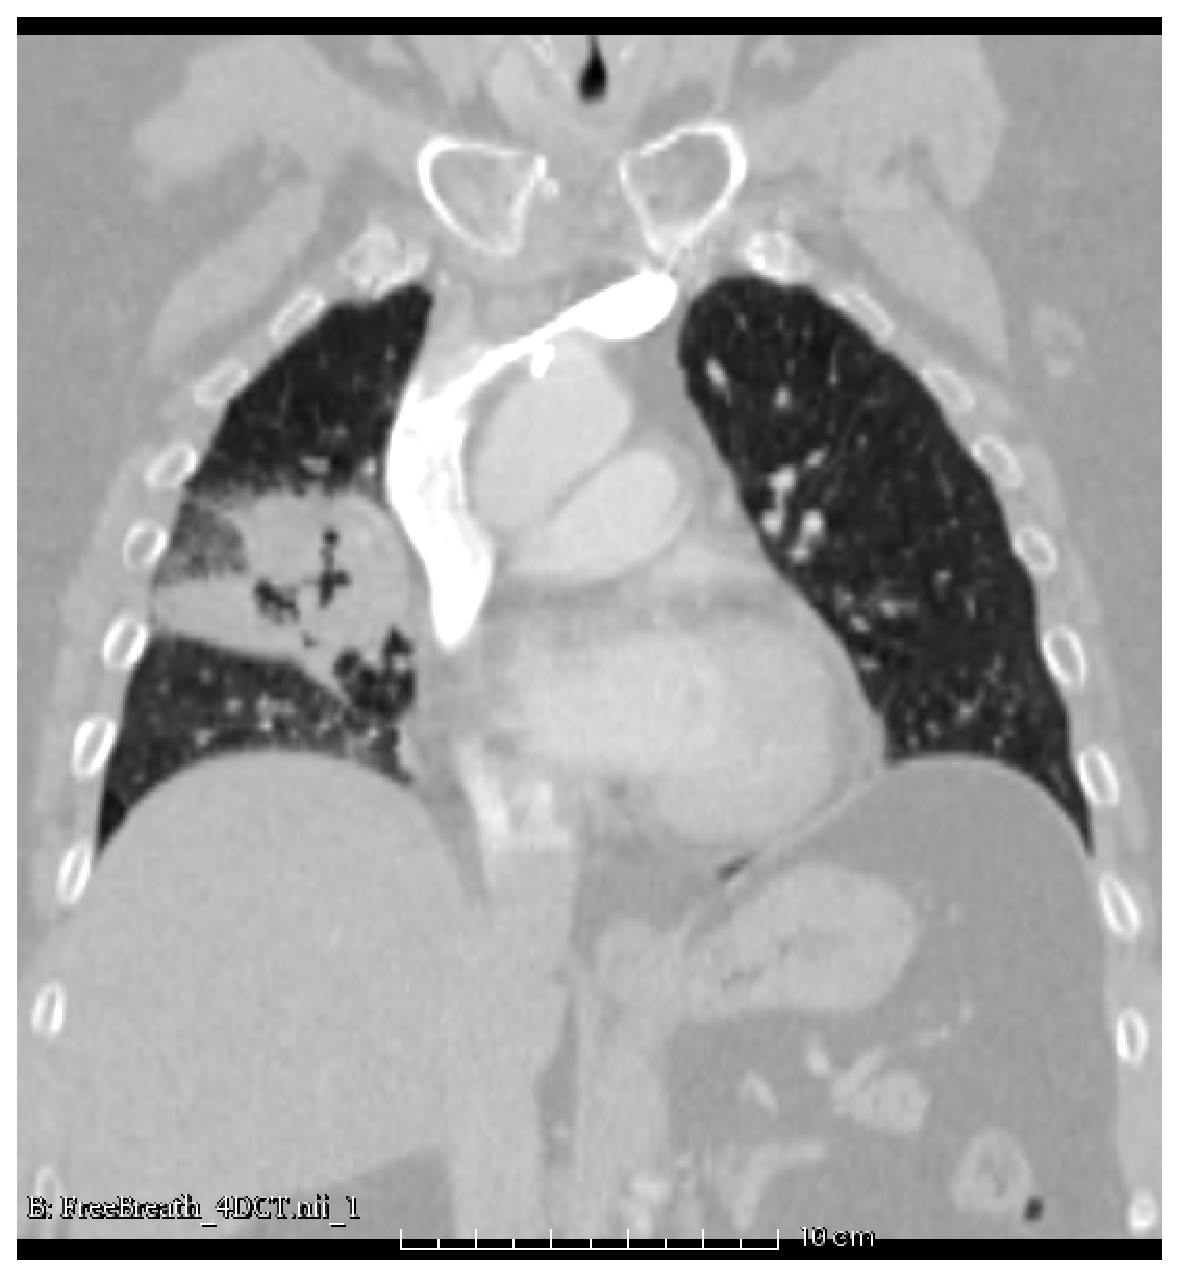
\includegraphics[trim={5 160 340 110},clip,width=1.1in, height=1.4in]{figs/ct} &
%    
\includegraphics[trim={5 150 300 100},clip,width=1.1in, height=1.4in]{figs/pass} &
%    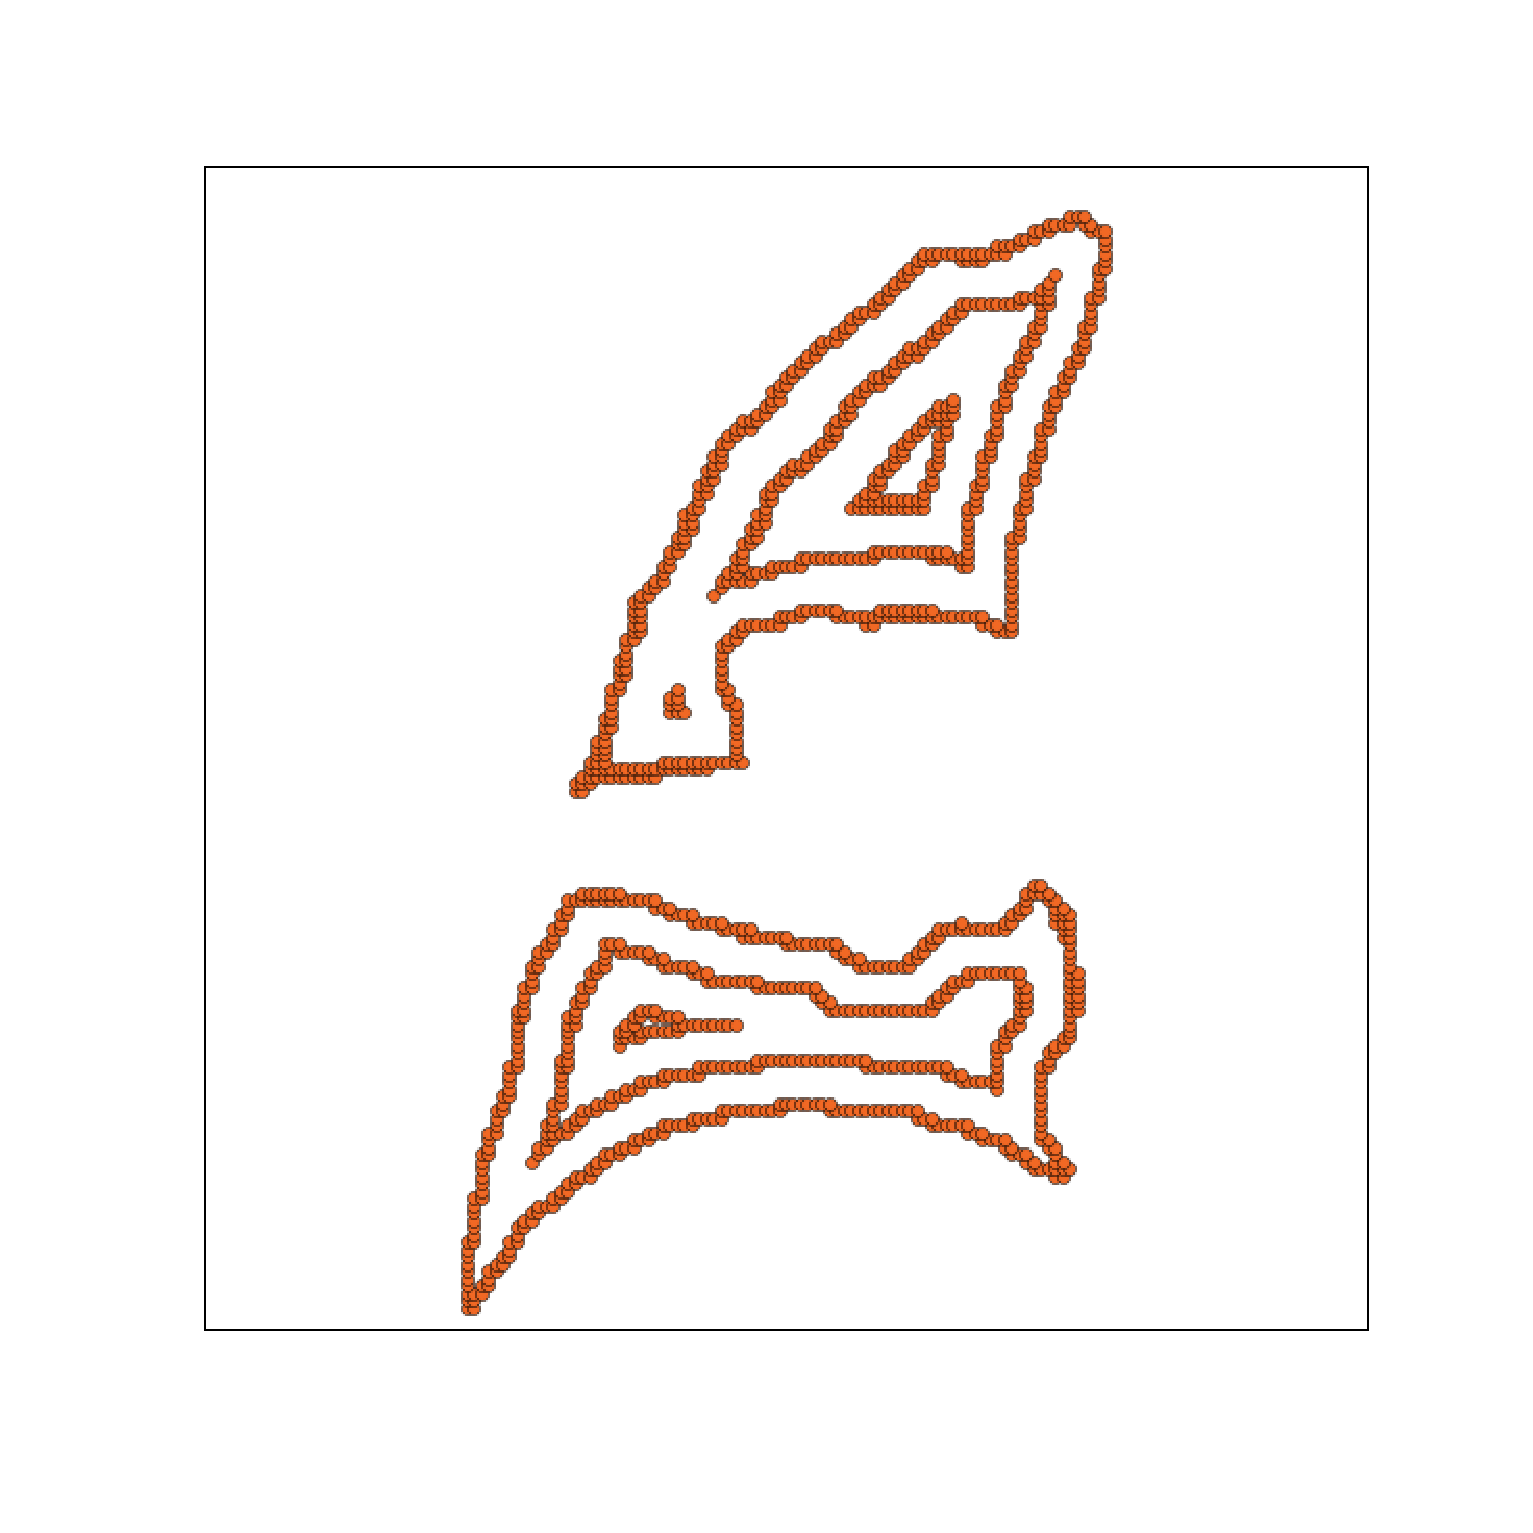
\includegraphics[trim={150 100 150 100},clip,width=1.1in]{figs/points} &
%    \includegraphics[trim={150 100 150 100},clip,width=1.1in]{figs/tris_200} \\
%    \includegraphics[trim={150 100 150 100},clip,width=1.1in]{figs/tris_66} &
%    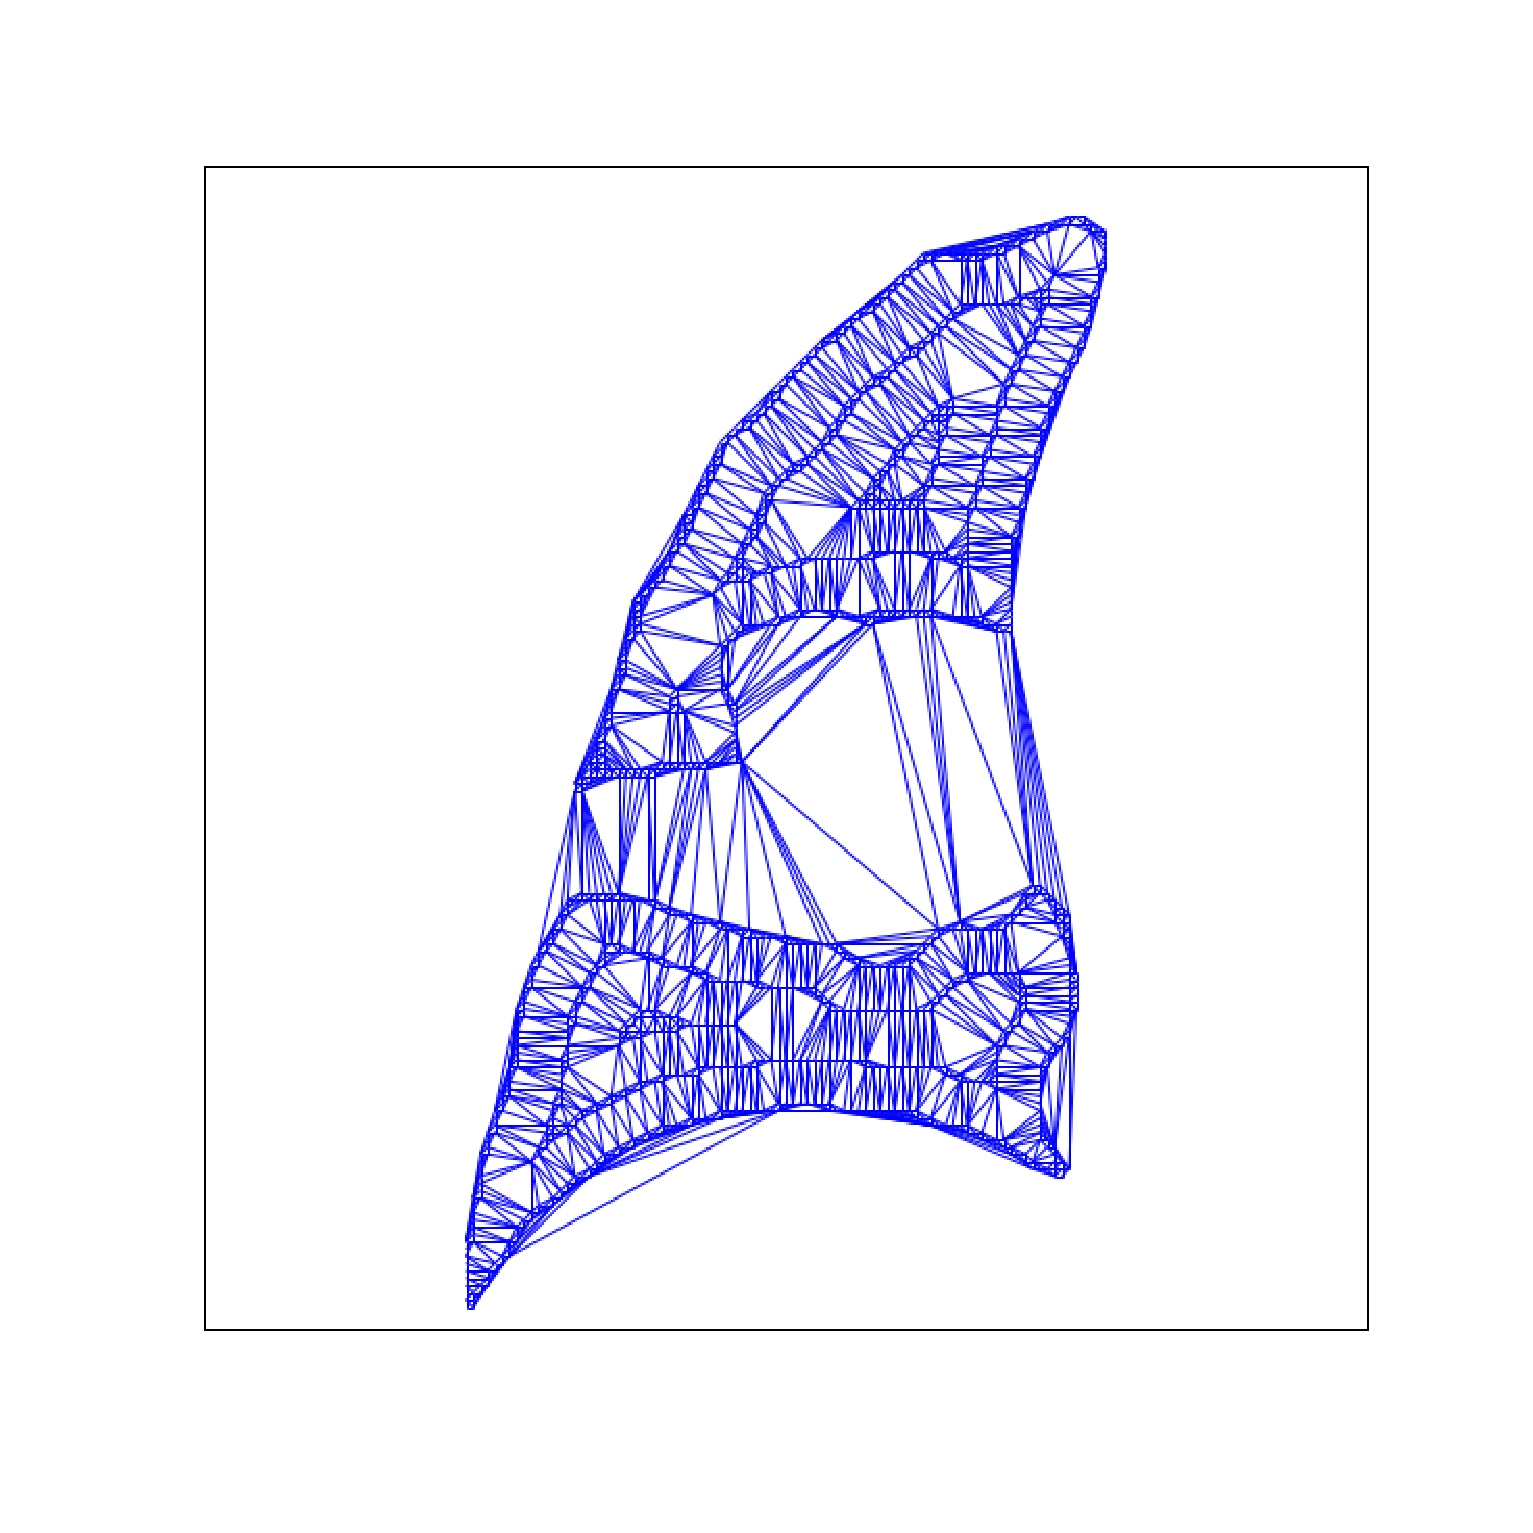
\includegraphics[trim={150 100 150 100},clip,width=1.1in]{figs/tris_50} &
%    \includegraphics[trim={150 100 150 100},clip,width=1.1in]{figs/tris_33} & 
%    \includegraphics[trim={150 100 150 100},clip,width=1.1in]{figs/tris_15} \\
%  \end{tabular}
  \caption{~\ref{fig:tris_CT} CT image, ~\ref{fig:tris_Mask} initial mask, ~\ref{fig:tris_points} point set used to represent mask, ~\ref{fig:tris_alpha_200} - ~\ref{fig:tris_alpha_15} Delaunay triangles that compose the alpha shape for decreasing alpha values. Note: this is a 2D example for illustrative purposes, the actual method is performed in 3D with tetrahedrons instead of triangles. }
  \label{fig:tris}
\end{figure}


\begin{figure}[t]
  \centering
    \subfigure[$\alpha = 200$]{
    \includegraphics[trim={200 5 200 5},clip, width=1.3in]{figs/alpha200} 
    \label{fig:img_alpha200}
    }
    \subfigure[$\alpha = 25$]{
    \includegraphics[trim={200 5 200 5},clip, width=1.3in]{figs/alpha25}
    \label{fig:img_alpha25}
    }
    \subfigure[$\alpha = 9$]{
    \includegraphics[trim={200 5 200 5},clip, width=1.3in]{figs/alpha9} 
    \label{fig:img_alpha9}
    }
  \caption{Alpha shape segmentation for different $\alpha$}
  \label{fig:alphashapes}
\end{figure}
%
\subsection{Graph Search}
%
The alpha shape generally over segments the mediastinum as a result of the non-convex shape. This could be eliminated by reducing $\alpha$, however then we way remove tumor regions as well. To reduce the mediastinum over segmentation, we use a graph search framework. The method will only briefly be described here, see~\cite{li2006} for a detailed description of the method. 

The graph search method requires a shape prior, here we use the alpha shape from the previous step as the shape prior. A graph $G(E,V)$ consisting of node set $V$ and edge set $E$ is built in a margin around the shape prior. The nodes have an associated cost reflecting the unlikeliness that it belongs to the lung surface. We use the inverse gradient of the CT image for the cost, as the lung surface has a high image gradient. Edges are used to enforce smoothness constraints, or how much the topology of the resulting segmentation can deviate from the shape prior. The globally optimal surface is obtained by using a maximum flow algorithm on a closely derived graph. 
 

%
\section{Data Sets and Experimental Setup}
%
In this study we used breath-hold thoracic CT scans from twelve lung cancer subjects about to undergo radiation therapy. All scans were gathered under a protocol approved by the 
XXXXXXXXXXX YYYYYYY 
%University of Iowa 
Institutional Review Board 
%(IRB 200905703). 
(IRB ZZZZZZZZZ).
All images were resampled to obtain $1\times{}1\times{}1$ mm$^3$ voxels. Subjects were chosen that had at least one large tumor. 

Out method was evaluated by comparing to ground truth segmentations generated by a radiation therapy physicist using the MimVista 6.4.7 software (MIM Software, Cleveland, OH). The DICE coefficient was used for a metric of volume overlap. Additionally, the average unsigned symmetric surface distance was used to measure the distance between the segmentation boundaries. The analysis was performed on both left and right lungs of all subjects. Additionally, we repeated the analysis with only considering the lung containing the tumor.


The proposed method was implemented using the jupyter notebook \cite{PER-GRA:2007} rapid prototyping environment,  algorithms from ITK\cite{johnson2015itk} python wrapped in SimpleITK \cite{10.3389/fninf.2013.00045} in coordination with vtkDelaunay3D from VTK (www.vtk.org).


%
\section{Results}
%

Figure ~\ref{fig:resultseg} shows the final segmentation for four subjects. 
\todo[author=HJ,inline]{Hard to see blue contour, ask Prof. Johnson if we can make contour thicker in Slicer.}

\begin{figure}[t]
  \centering
    \subfigure[]{
    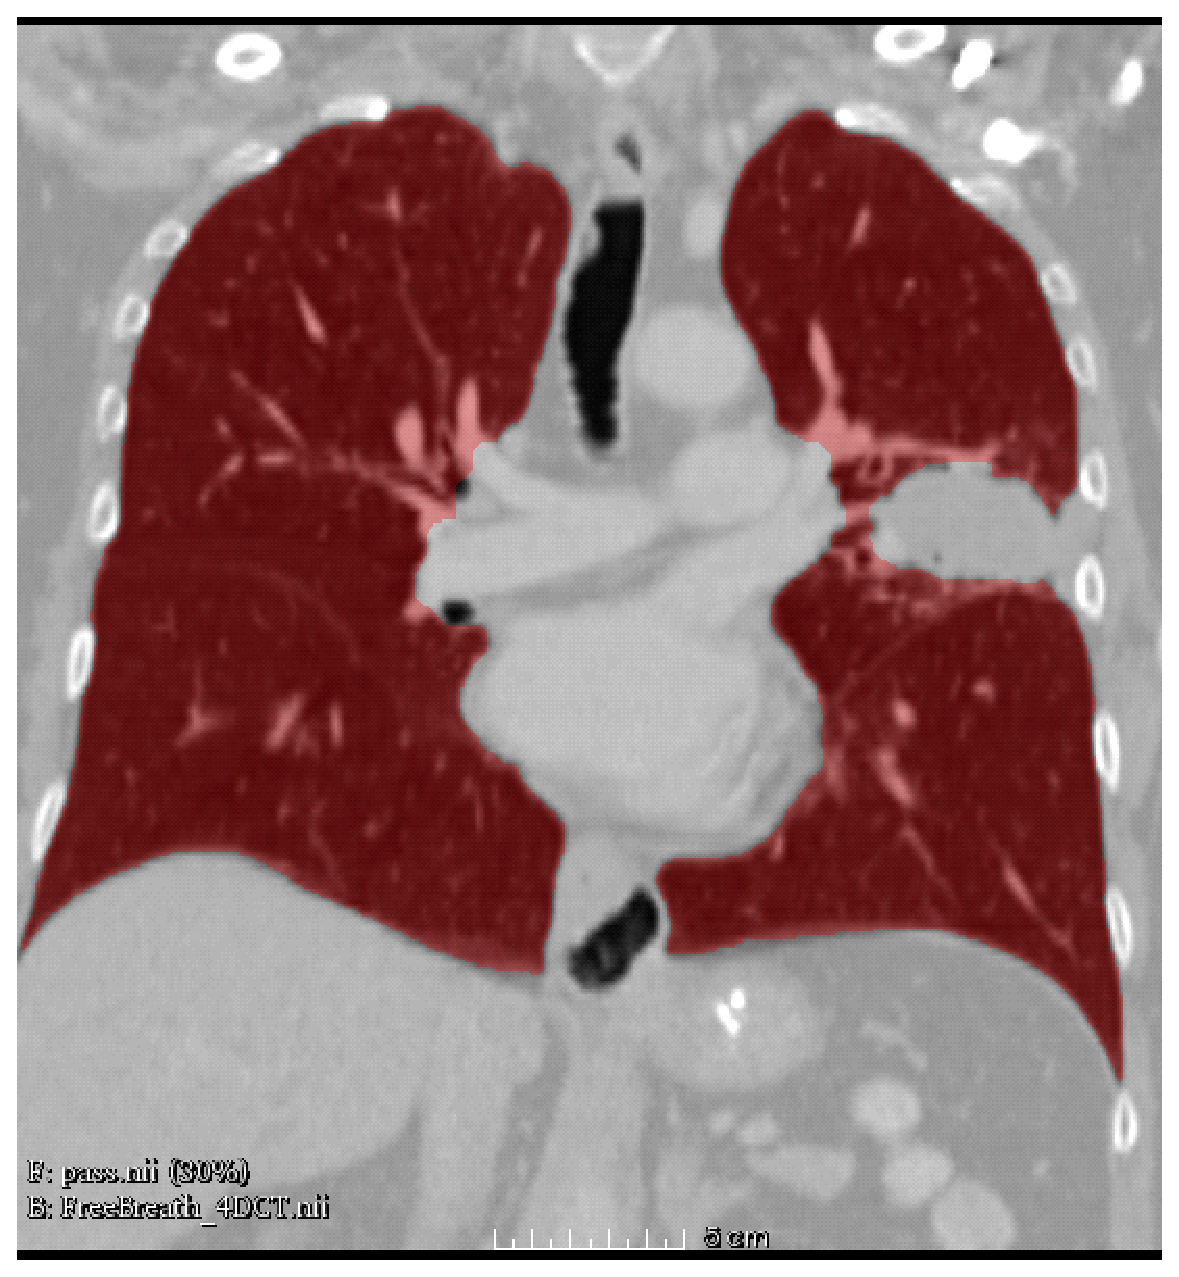
\includegraphics[width=1in]{figs/PFS-002_pass}
    \label{fig:PFS-002_pass}
    }
    \subfigure[]{
    \includegraphics[width=1in]{figs/PFS-002_alpha}
    \label{fig:PFS-002_alpha}
    }
    \subfigure[]{
    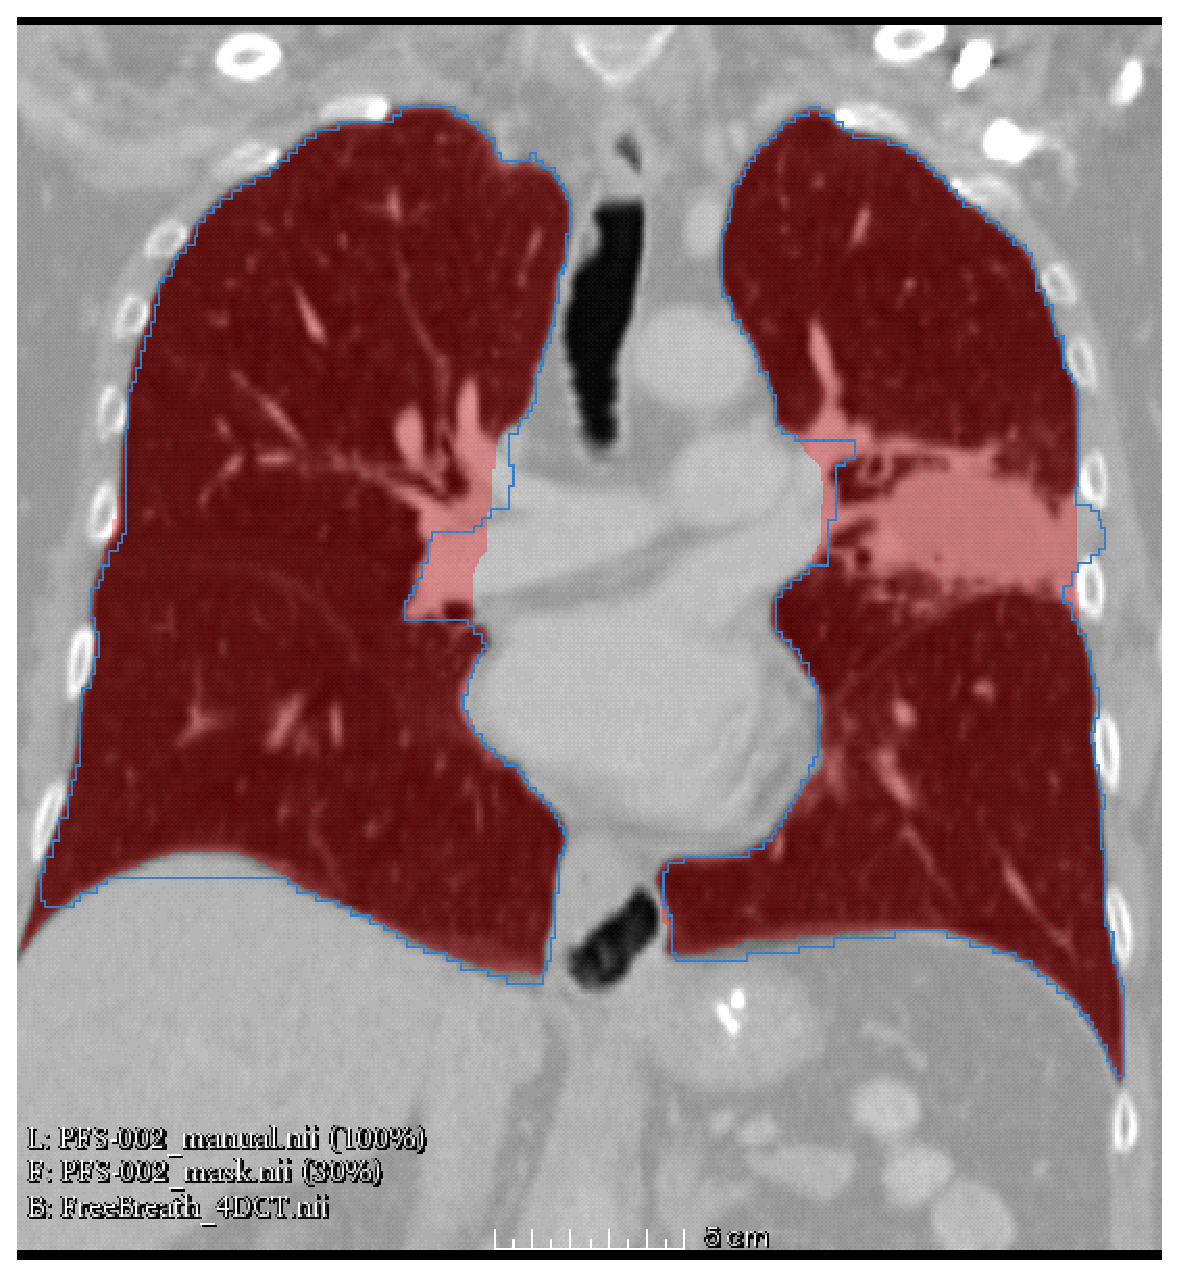
\includegraphics[width=1in]{figs/PFS-002_final}
    \label{fig:PFS-002_final}
    }\\
    \subfigure[]{
    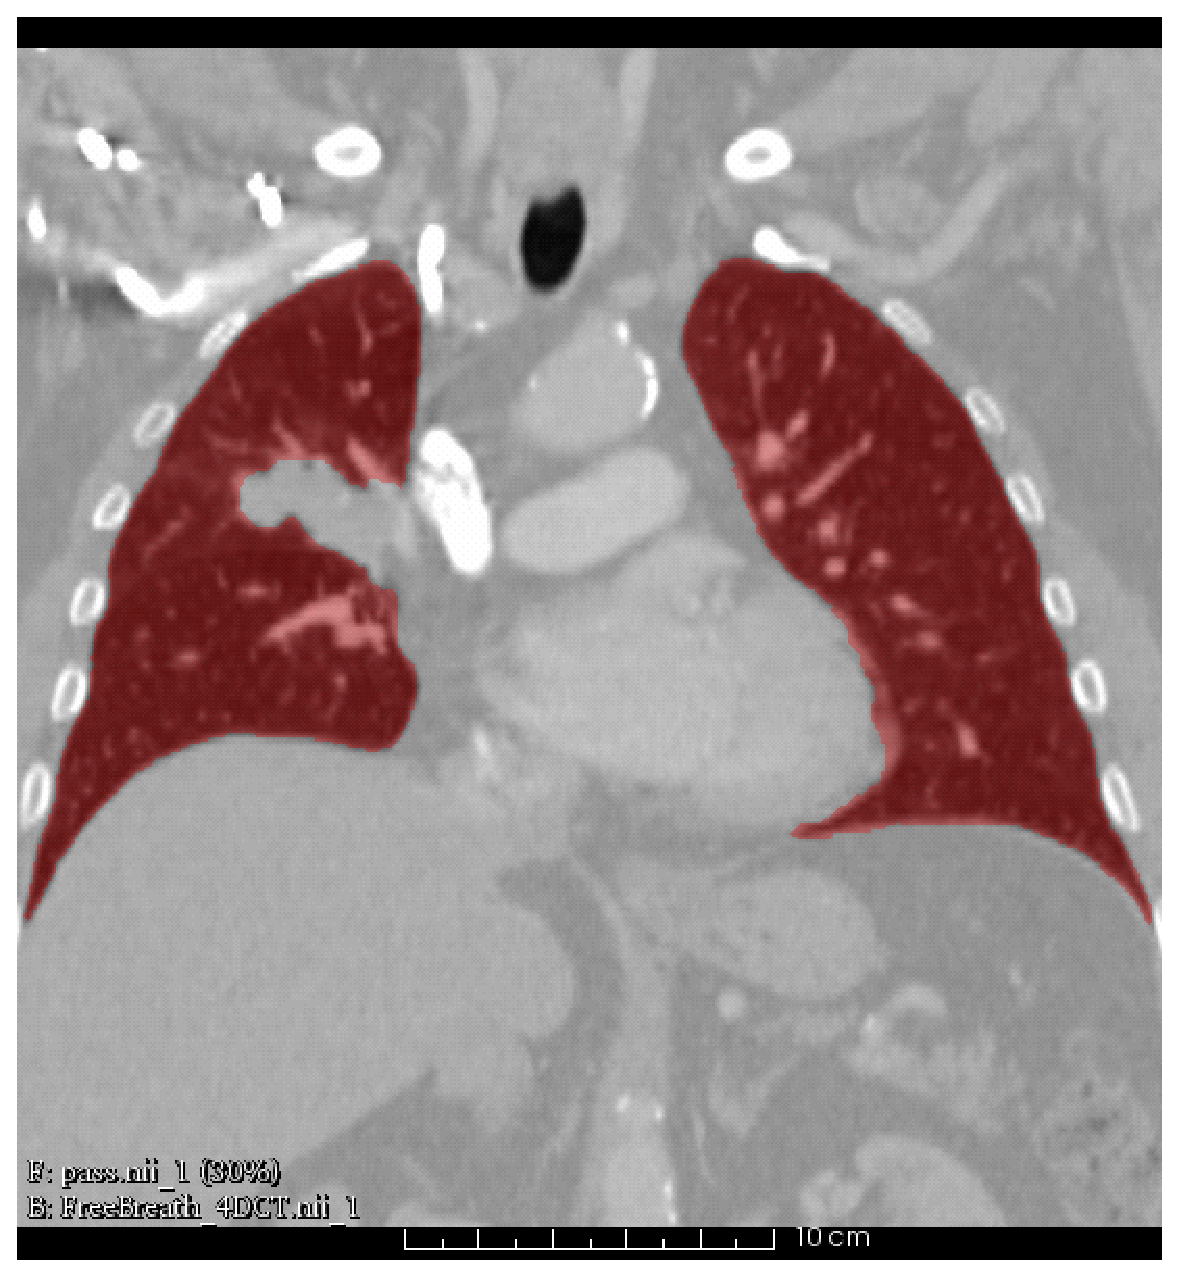
\includegraphics[width=1in]{figs/PFS-011_pass}
    \label{fig:PFS-011_pass}
    }
    \subfigure[]{
    \includegraphics[width=1in]{figs/PFS-011_alpha}
    \label{fig:PFS-011_alpha}
    }
    \subfigure[]{
    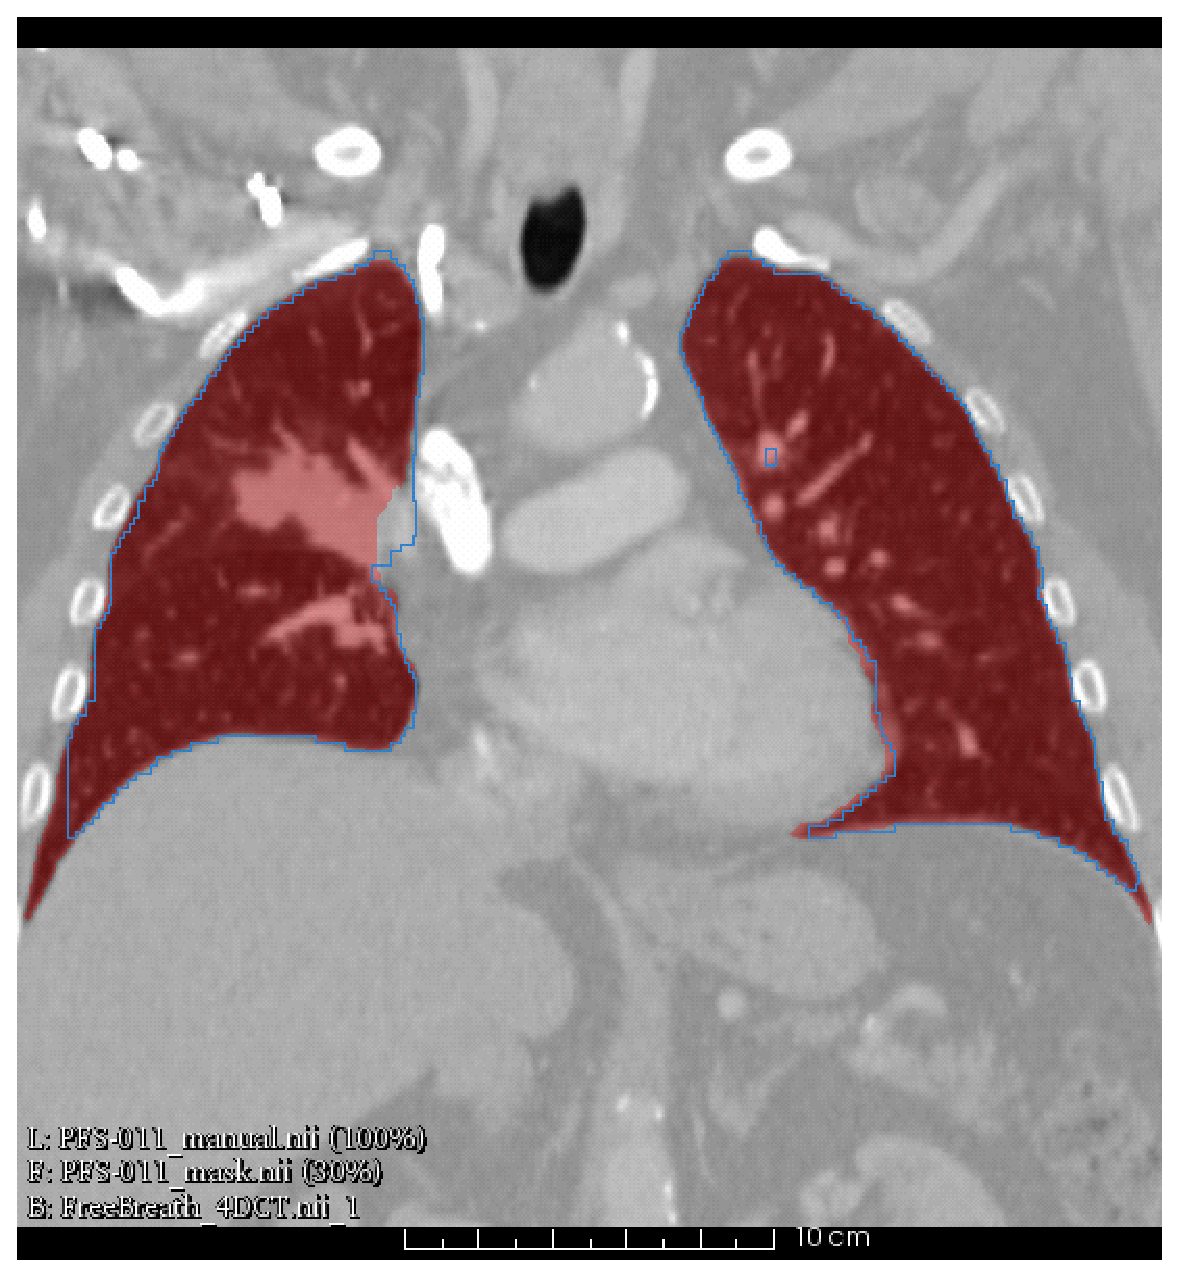
\includegraphics[width=1in]{figs/PFS-011_final}
    \label{fig:PFS-011_final}
    }\\
    \subfigure[]{
    \includegraphics[width=1in]{figs/PFS-020_pass}
    \label{fig:PFS-020_pass}
    }
    \subfigure[]{
    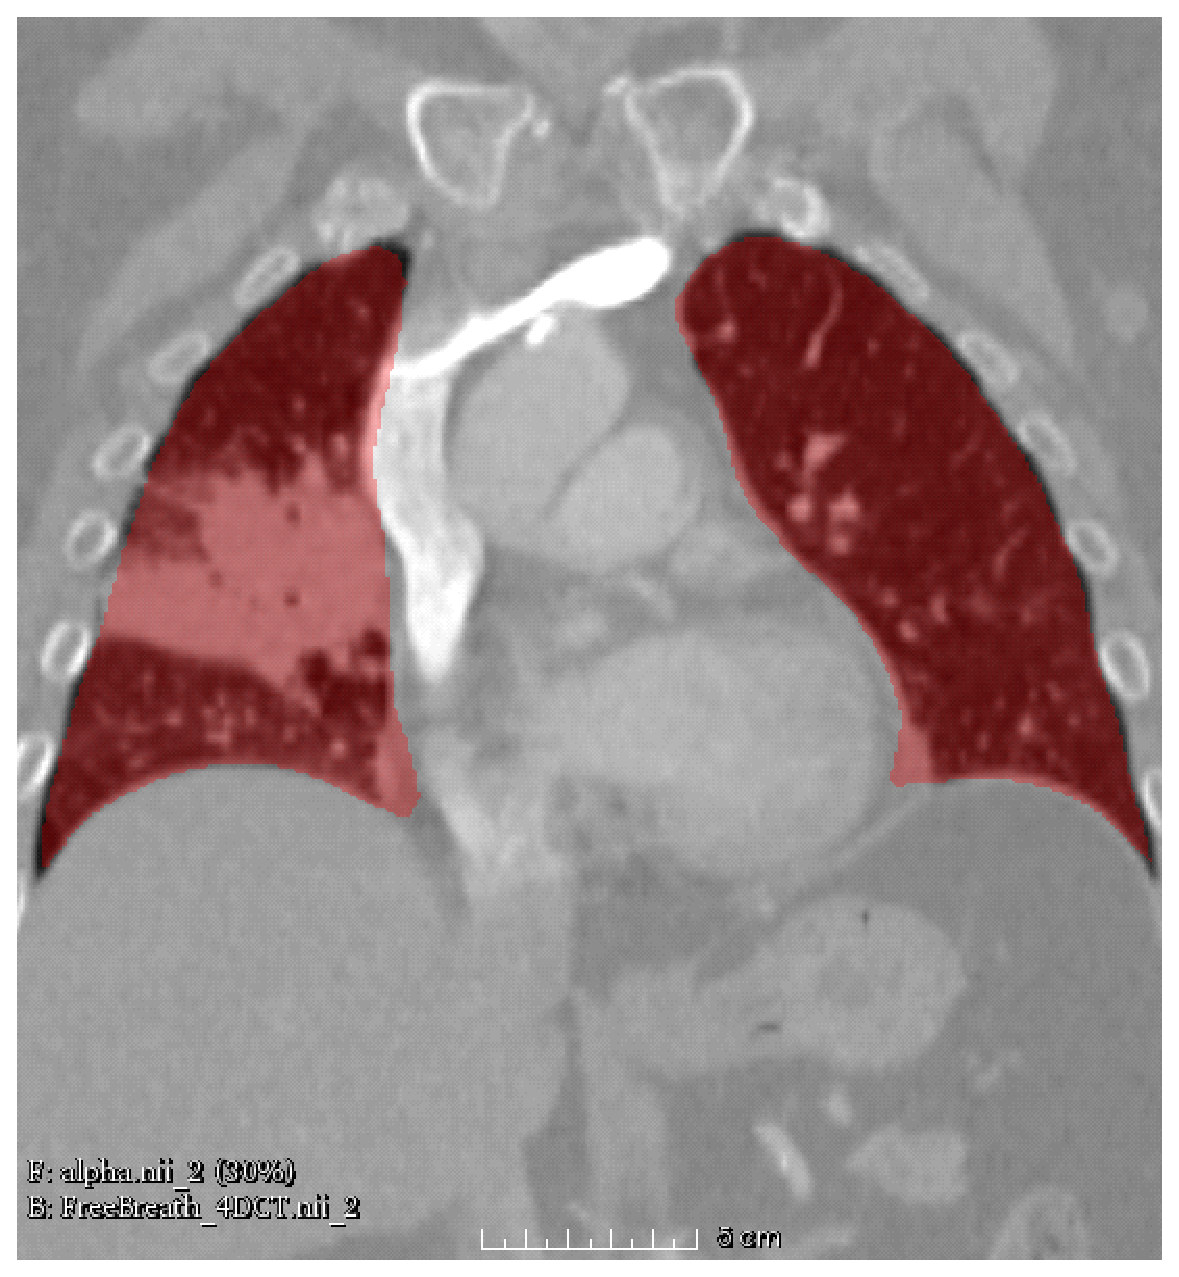
\includegraphics[width=1in]{figs/PFS-020_alpha}
    \label{fig:PFS-020_alpha}
    }
    \subfigure[]{
    \includegraphics[width=1in]{figs/PFS-020_final}
    \label{fig:PFS-020_final}
    }\\
    \subfigure[]{
    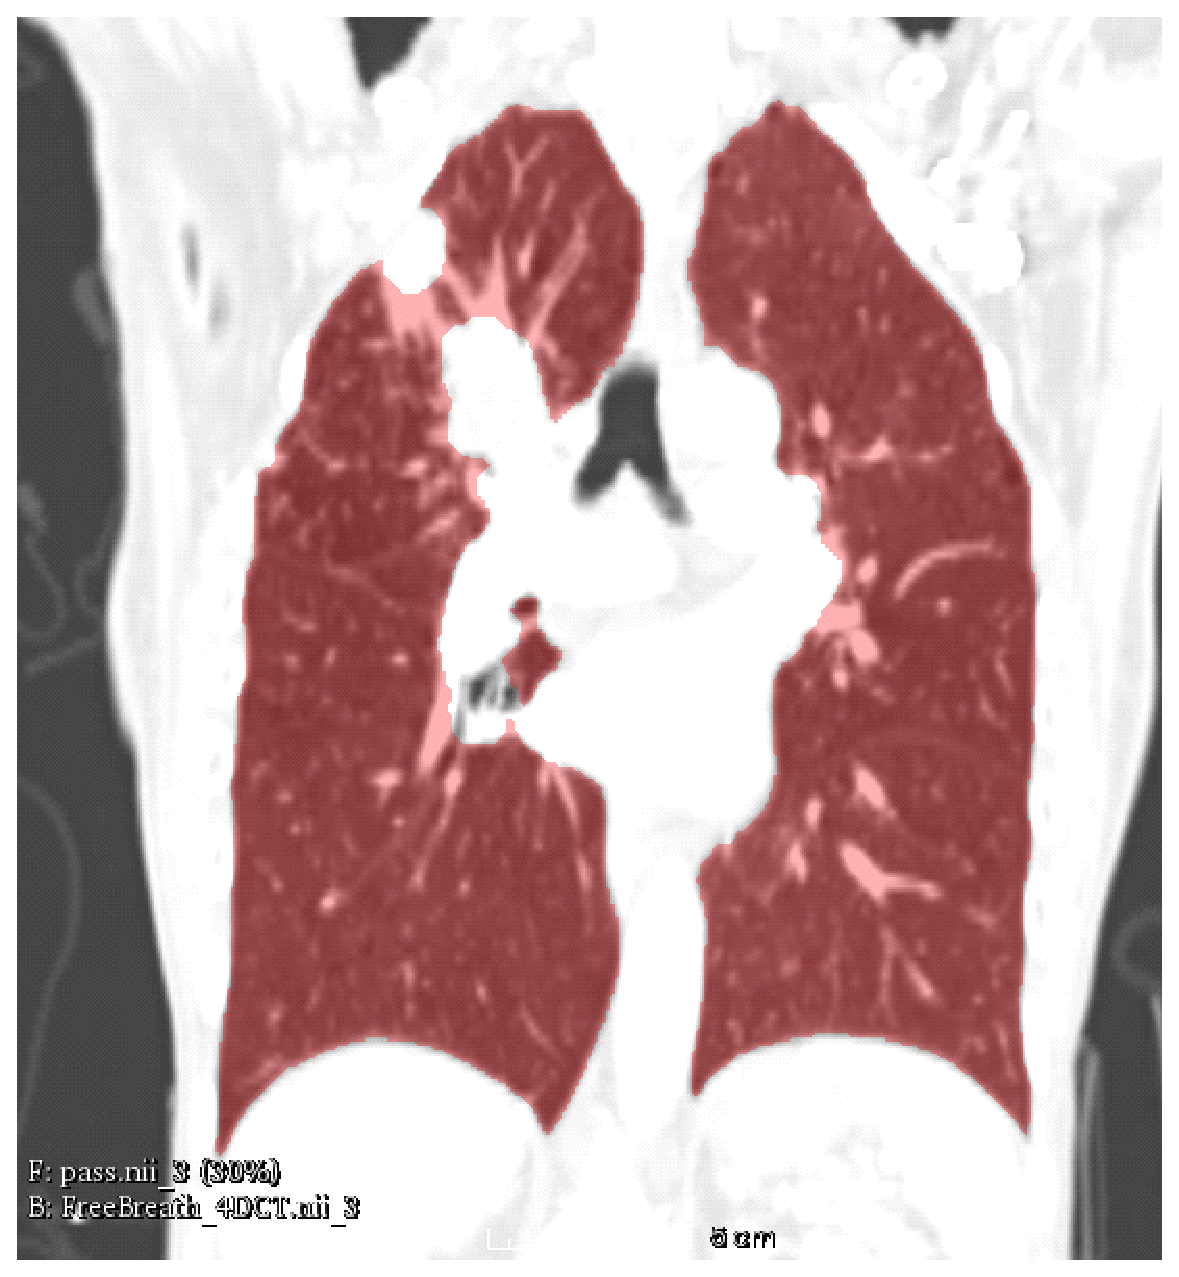
\includegraphics[width=1in]{figs/PFS-031_pass}
    \label{fig:PFS-031_pass}
    }
    \subfigure[]{
    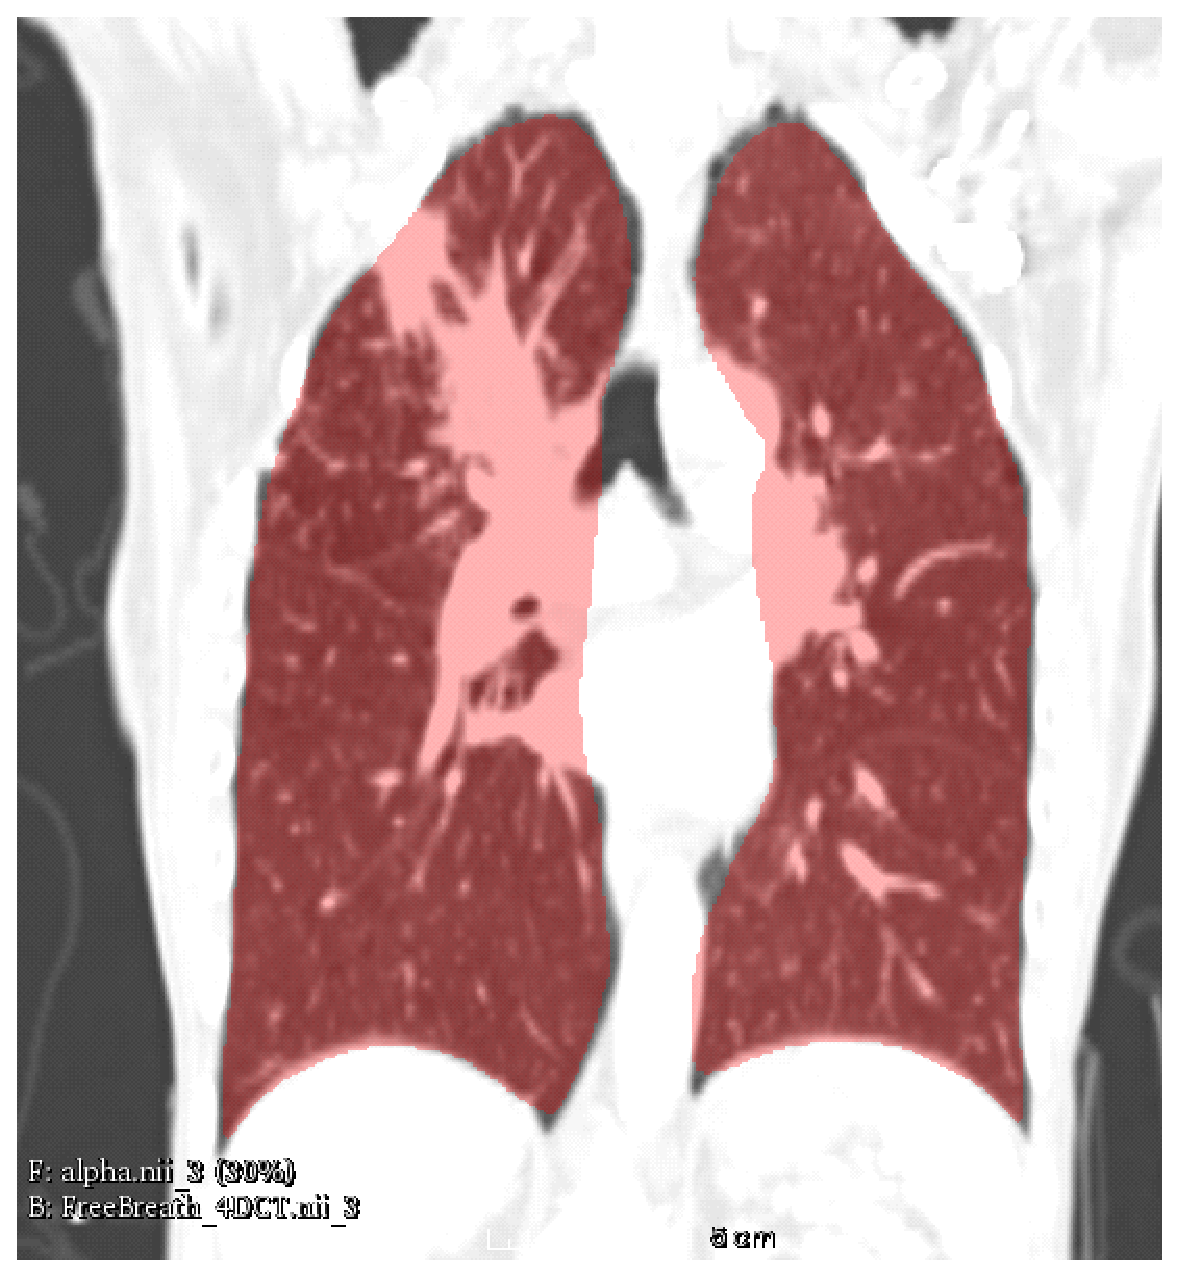
\includegraphics[width=1in]{figs/PFS-031_alpha}
    \label{fig:PFS-031_alpha}
    }
    \subfigure[]{
    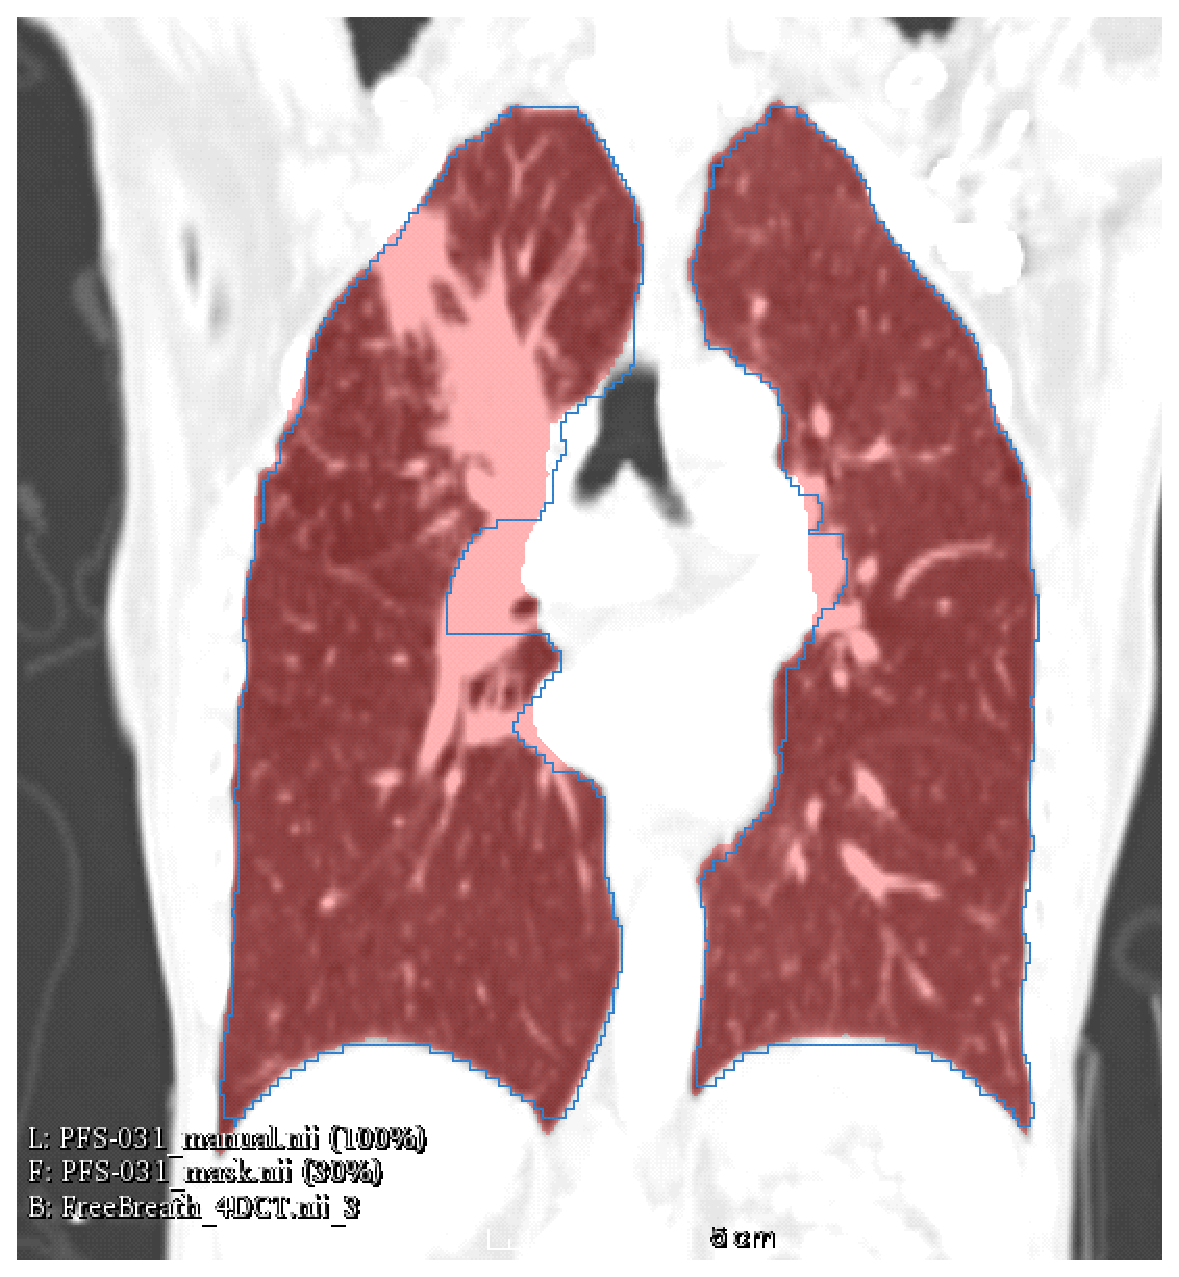
\includegraphics[width=1in]{figs/PFS-031_final}
    \label{fig:PFS-031_final}
    }

  \caption{Result for four subjects. First column shows the initial mask. Second column shows the alpha shape of the initial mask. The third column shows the final result in red along with the manual segmentation outlined in blue}
  \label{fig:resultseg}
\end{figure}

Figure ~\ref{fig:dice} and ~\ref{fig:dist} shows DICE coefficient and average unsigned symmetric surface distance for left and right lungs of all subjects.
\begin{figure}[t]
  \centering
    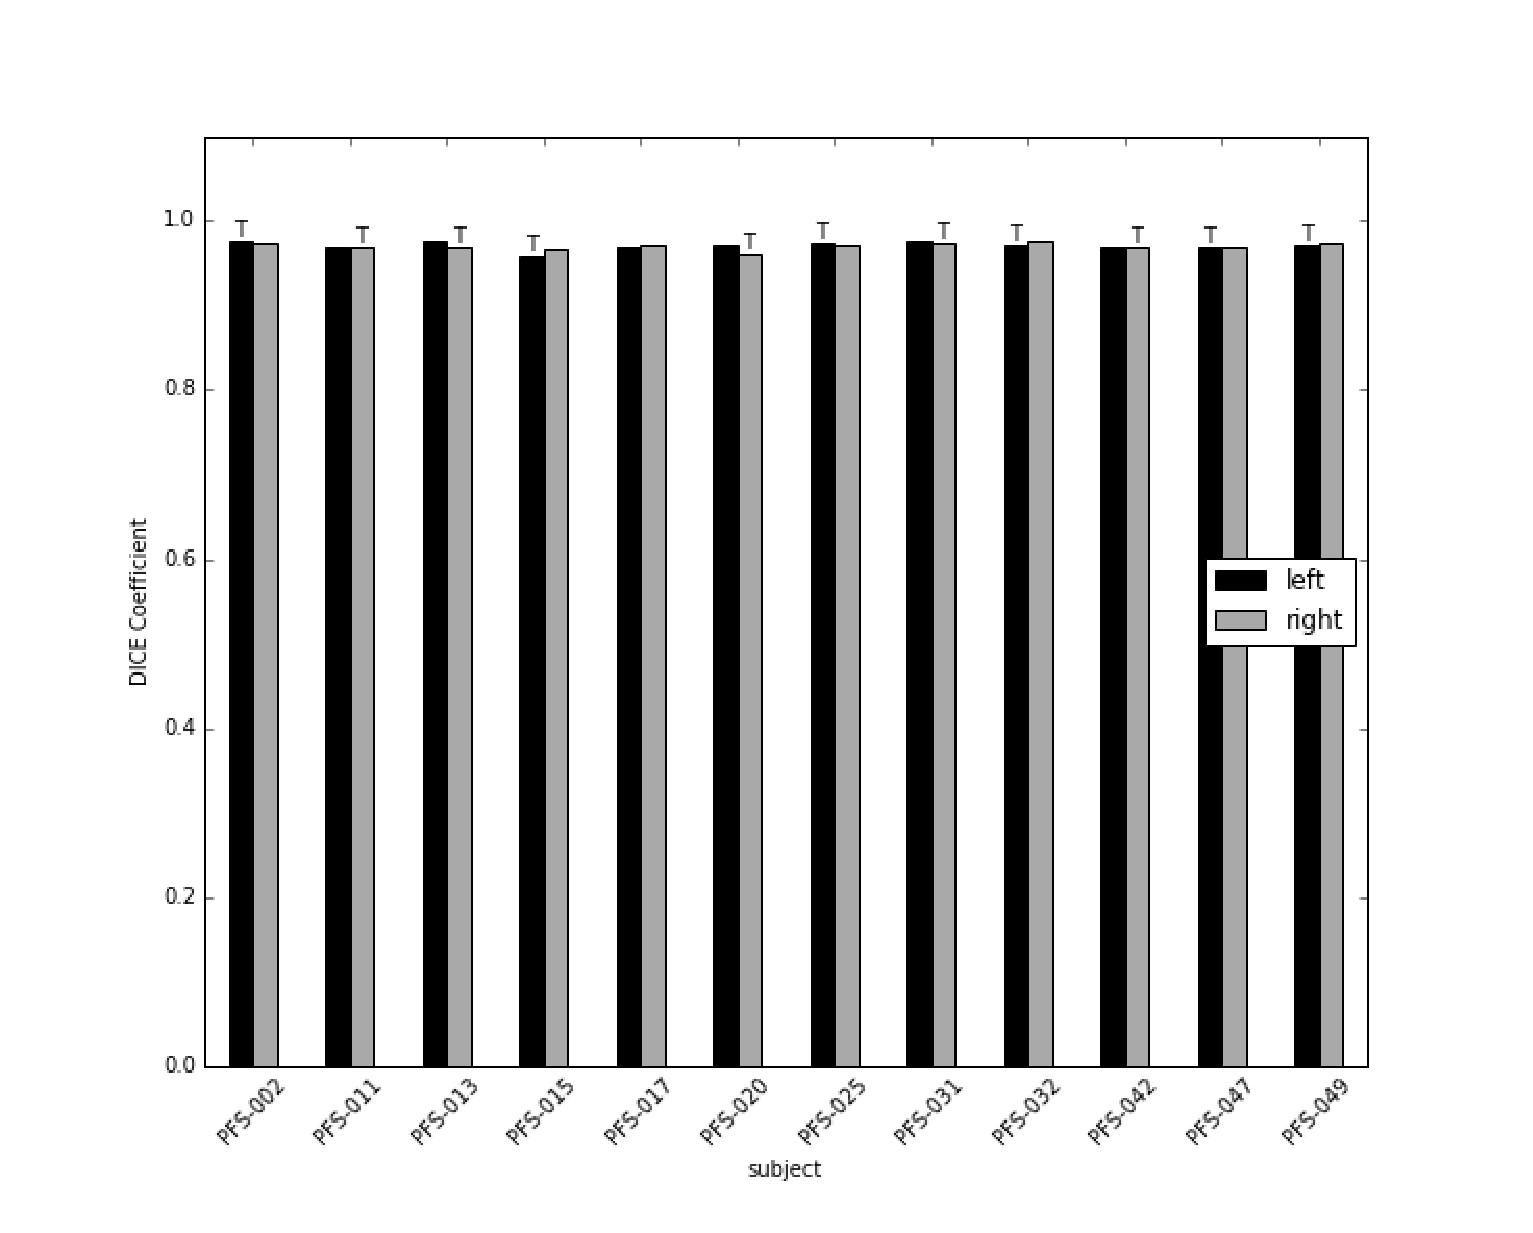
\includegraphics[width=4.5in]{figs/dice}
  \caption{DICE coefficient for all subjects. "o" indicates lungs with tumors.}
  \label{fig:dice}
\end{figure}

\begin{figure}[t]
  \centering
    \includegraphics[width=4.5in]{figs/distUnsignSym}
  \caption{Average unsigned symmetric surface distance for all subjects. "o" indicates lungs with tumors.}
  \label{fig:dist}
\end{figure}

\iffalse
Table ~\ref{tab:results} shows the DICE coefficient and surface distance for left and right lungs of each subject. 


% define table layout and column spacing here
\newlength\intercol
\setlength\intercol{15pt}
\newlength\betweenwidth
\setlength\betweenwidth{10pt}
\newcommand\icspace{@{\hspace\intercol}}
\newcommand\inspace{@{\hspace\betweenwidth}}
\newcommand\MC[1]{\multicolumn{2}{c\icspace}{#1}}
\newcommand\MClast[1]{\multicolumn{2}{c}{#1}}

\begin{table}
  \centering
  \begin{tabular}{c@{\hspace{20pt}} c \inspace c \icspace c \inspace c \icspace c \inspace c}
    \toprule
    Subject & \MC{DICE}   & \MC{Surface Distance}  & \MC{HD}\\
            & Left & Right & Left & Right & Left & Right \\
    \midrule
    A & XXX & XXX & XXX & XXX & XXX & XXX \\
    B & XXX & XXX & XXX & XXX & XXX & XXX \\
    C & XXX & XXX & XXX & XXX & XXX & XXX \\
    D & XXX & XXX & XXX & XXX & XXX & XXX \\
    E & XXX & XXX & XXX & XXX & XXX & XXX \\
    F & XXX & XXX & XXX & XXX & XXX & XXX \\
    G & XXX & XXX & XXX & XXX & XXX & XXX \\
    H & XXX & XXX & XXX & XXX & XXX & XXX \\
    I & XXX & XXX & XXX & XXX & XXX & XXX \\
    J & XXX & XXX & XXX & XXX & XXX & XXX \\
    K & XXX & XXX & XXX & XXX & XXX & XXX \\
    L & XXX & XXX & XXX & XXX & XXX & XXX \\
    \midrule
    Mean & XXX & XXX & XXX & XXX & XXX & XXX \\
    \bottomrule \\
  \end{tabular}
  \caption{Results for proposed method compared to manual segmentations.}
  \label{tab:results}
\end{table}
\fi

\iffalse
Figure ~\ref{fig:steps} shows the resulting segmentation at each step of the method for one subject.



\begin{figure}[t]
  \centering
    \subfigure[Initial Mask]{
    \includegraphics[trim={200 5 200 5},clip, width=1.3in]{figs/step_pass}
    \label{fig:pass}
    }
    \subfigure[Alpha Shape]{
    \includegraphics[trim={200 5 200 5},clip, width=1.3in]{figs/step_alpha}
    \label{fig:alpha}
    }
    \subfigure[Graph Search]{
    \includegraphics[trim={200 5 200 5},clip, width=1.3in]{figs/step_osf}
    \label{fig:osf}
    }
  \caption{Result after each step of the proposed method.}
  \label{fig:steps}
\end{figure}
\fi





%
\section{Discussion}
%

The method shows good results with a DICE coefficient of 0.970 and average unsigned symmetric surface distance of 0.809 mm for all subjects. This surface distance is on the sub-voxel level. Additionally, we split the lungs into tumor and non-tumor groups. The DICE coefficient was 0.967 and 0.971 for tumor and non-tumor groups, respectively. The unsigned symmetric surface distance was 0.826 mm and 0.794 mm for tumor and non-tumor groups, respectively. A t-test was performed to compare the surface distance error for lungs with tumors and lungs without tumors and no significant difference was found (p-value = 0.540).

The experiments were run on a Linux machine with an Intel Xeon 2.27 GHz CPU and 48 GB of RAM. Generating the alpha shape and the graph search takes XXX and XXX minutes of computer time, respectively. The manual segmentation took on average 53 minutes per subject.

Our future directions involve learning the optimal alpha for a given subject rather than using the same alpha for all subject. Additionally, we plan to experiment with learning a spatially varying alpha to overcome over segmentation near the aorta.
%
\section{Summary}
%
We proposed a method for segmentation of lungs in the presence of large tumors. The method is utilizes an intensity based segmentation, alpha shapes, and a graph search framework. A DICE coefficient of 0.970 and a surface distance of 0.809 mm were achieved. The accurate lung segmentation with  inclusion of tumor regions is valuable for radiation therapy treatment planning and further quantitative analysis.
%
\section{Acknowledgments}
%
This work was supported in part by 
%NIH grant CA166703.
XXXXXXX XXXXXXXXXXX.


%
% ---- Bibliography ----
%
\bibliography{refs.bib}
\bibliographystyle{splncs03}







\clearpage
\addtocmark[2]{Author Index} % additional numbered TOC entry
\renewcommand{\indexname}{Author Index}
\printindex
\clearpage
\iffalse
\addtocmark[2]{Subject Index} % additional numbered TOC entry
\markboth{Subject Index}{Subject Index}
\renewcommand{\indexname}{Subject Index}
\input{subjidx.tex}
\fi
\end{document}
